\documentclass[border=2pt]{standalone}
\usepackage[T1]{fontenc}
\usepackage{newtxtext,newtxmath}
\usepackage{pifont,fontawesome5}
\usepackage{tikz}
\usetikzlibrary{arrows.meta,shadows}
\definecolor{hesp}{HTML}{4C72B0}
\definecolor{llm}{HTML}{DD8452}
\definecolor{env}{HTML}{8C8C8C}
\definecolor{ver}{HTML}{55A868}
\newcommand{\stepnum}[1]{\tikz[baseline=-0.6ex]\node[circle, fill=black, text=white, font=\scriptsize\bfseries, inner sep=0.8pt, minimum size=10pt] {#1};}
\begin{document}
\begin{tikzpicture}[font=\scriptsize,
  lab/.style={font=\scriptsize, inner sep=1pt},
  stage/.style={draw=black!70, dashed, line width=0.8pt, rounded corners=6pt},
  stagehead/.style={anchor=north west, font=\footnotesize\bfseries\itshape},
  card/.style={draw=#1, line width=0.7pt, fill=white, rounded corners=3pt, drop shadow={opacity=0.15, shadow xshift=0.4pt, shadow yshift=-0.4pt}},
  chip/.style={draw=black!40, fill=hesp!10, rounded corners=2pt, minimum width=1.44cm, minimum height=0.42cm, font=\scriptsize},
  doc/.style={draw=black!60, fill=white, minimum width=0.72cm, minimum height=0.9cm, line width=0.6pt},
  server/.style={draw=black!55, fill=black!8, minimum width=0.7cm, minimum height=0.8cm, rounded corners=1pt},
  flow/.style={-{Stealth[length=5pt]}, line width=0.8pt, draw=#1}]

% ---------- planner band (top)
\node[card=llm, minimum width=17.2cm, minimum height=0.95cm] (planner) at (8.9,8.55) {};
\node[anchor=west, font=\footnotesize\bfseries] at (0.45,8.72) {Local LLM planner};
\node[anchor=west, lab] at (0.45,8.35) {Llama-3.1-8B, served locally};
\node[anchor=west, lab, font=\scriptsize\ttfamily, text=black!80] at (4.15,8.72)
  {\{"kind": "action", "action\_id": "auth\_log"\} \ \ \textrm{(3 of 3 decisions)}};
\node[anchor=west, lab] at (4.15,8.35) {proposes probes but never issues a verdict; it sees no ranking};
\draw[flow=llm] (7.95,8.07) -- (7.95,7.45) node[midway, right, lab, text=llm!90!black] {propose};
\draw[flow=llm, dashed] (14.9,8.07) -- (14.9,7.45) node[midway, right, lab, text=llm!90!black] {finish (never used)};

% ---------- alert
\node[doc] (alert) at (0.75,4.9) {};
\draw[fill=red!75!black] (0.75,5.05) -- (0.97,4.68) -- (0.53,4.68) -- cycle;
\node[text=white, font=\tiny\bfseries] at (0.75,4.79) {!};
\node[lab, align=center] at (0.75,4.15) {alert\\sec-base-02};
\draw[flow=black!60] (1.2,4.9) -- (1.85,4.9);

% ---------- stage 1: ledger
\draw[stage] (1.9,1.55) rectangle (7.1,7.35);
\node[stagehead] at (2.0,7.12) {\stepnum{1} Hypothesis Ledger};
\node[lab] at (4.73,6.46) {prior};
\node[lab] at (5.39,6.46) {IPs};
\node[lab] at (6.05,6.46) {HTTP};
\node[lab] at (6.71,6.46) {admin};
\node[lab, anchor=east] at (4.34,5.99) {credential stuffing};
\draw[draw=black!25, fill=hesp!9] (4.40,5.80) rectangle (5.06,6.18);
\node[lab, text=black!75] at (4.73,5.99) {.11};
\draw[draw=black!25, fill=white] (5.06,5.80) rectangle (5.72,6.18);
\node[lab, text=black!75] at (5.39,5.99) {0};
\draw[draw=black!25, fill=white] (5.72,5.80) rectangle (6.38,6.18);
\node[lab, text=black!75] at (6.05,5.99) {0};
\draw[draw=black!25, fill=white] (6.38,5.80) rectangle (7.04,6.18);
\node[lab, text=black!75] at (6.71,5.99) {0};
\node[lab, anchor=east] at (4.34,5.61) {SQL injection};
\draw[draw=black!25, fill=hesp!9] (4.40,5.42) rectangle (5.06,5.80);
\node[lab, text=black!75] at (4.73,5.61) {.11};
\draw[draw=black!25, fill=hesp!20] (5.06,5.42) rectangle (5.72,5.80);
\node[lab, text=black!75] at (5.39,5.61) {.24};
\draw[draw=black!25, fill=white] (5.72,5.42) rectangle (6.38,5.80);
\node[lab, text=black!75] at (6.05,5.61) {0};
\draw[draw=black!25, fill=white] (6.38,5.42) rectangle (7.04,5.80);
\node[lab, text=black!75] at (6.71,5.61) {0};
\node[lab, anchor=east, text=red!75!black, font=\scriptsize\bfseries] at (4.34,5.23) {exposed admin panel};
\draw[draw=black!25, fill=hesp!9] (4.40,5.04) rectangle (5.06,5.42);
\node[lab, text=black!75] at (4.73,5.23) {.11};
\draw[draw=black!25, fill=hesp!20] (5.06,5.04) rectangle (5.72,5.42);
\node[lab, text=black!75] at (5.39,5.23) {.24};
\draw[draw=black!25, fill=hesp!28] (5.72,5.04) rectangle (6.38,5.42);
\node[lab, text=black!75] at (6.05,5.23) {.33};
\draw[draw=red!80!black, line width=0.9pt, fill=hesp!82] (6.38,5.04) rectangle (7.04,5.42);
\node[lab, text=white] at (6.71,5.23) {.97};
\node[lab, anchor=east] at (4.34,4.85) {authorized scan};
\draw[draw=black!25, fill=hesp!9] (4.40,4.66) rectangle (5.06,5.04);
\node[lab, text=black!75] at (4.73,4.85) {.11};
\draw[draw=black!25, fill=white] (5.06,4.66) rectangle (5.72,5.04);
\node[lab, text=black!75] at (5.39,4.85) {0};
\draw[draw=black!25, fill=white] (5.72,4.66) rectangle (6.38,5.04);
\node[lab, text=black!75] at (6.05,4.85) {0};
\draw[draw=black!25, fill=white] (6.38,4.66) rectangle (7.04,5.04);
\node[lab, text=black!75] at (6.71,4.85) {0};
\node[lab, anchor=east] at (4.34,4.47) {monitoring FP};
\draw[draw=black!25, fill=hesp!9] (4.40,4.28) rectangle (5.06,4.66);
\node[lab, text=black!75] at (4.73,4.47) {.11};
\draw[draw=black!25, fill=white] (5.06,4.28) rectangle (5.72,4.66);
\node[lab, text=black!75] at (5.39,4.47) {0};
\draw[draw=black!25, fill=white] (5.72,4.28) rectangle (6.38,4.66);
\node[lab, text=black!75] at (6.05,4.47) {0};
\draw[draw=black!25, fill=white] (6.38,4.28) rectangle (7.04,4.66);
\node[lab, text=black!75] at (6.71,4.47) {0};
\node[lab, anchor=east] at (4.34,4.09) {insider exfiltration};
\draw[draw=black!25, fill=hesp!9] (4.40,3.90) rectangle (5.06,4.28);
\node[lab, text=black!75] at (4.73,4.09) {.11};
\draw[draw=black!25, fill=white] (5.06,3.90) rectangle (5.72,4.28);
\node[lab, text=black!75] at (5.39,4.09) {0};
\draw[draw=black!25, fill=white] (5.72,3.90) rectangle (6.38,4.28);
\node[lab, text=black!75] at (6.05,4.09) {0};
\draw[draw=black!25, fill=white] (6.38,3.90) rectangle (7.04,4.28);
\node[lab, text=black!75] at (6.71,4.09) {0};
\node[lab, anchor=east] at (4.34,3.71) {vulnerable component};
\draw[draw=black!25, fill=hesp!9] (4.40,3.52) rectangle (5.06,3.90);
\node[lab, text=black!75] at (4.73,3.71) {.11};
\draw[draw=black!25, fill=hesp!20] (5.06,3.52) rectangle (5.72,3.90);
\node[lab, text=black!75] at (5.39,3.71) {.24};
\draw[draw=black!25, fill=hesp!28] (5.72,3.52) rectangle (6.38,3.90);
\node[lab, text=black!75] at (6.05,3.71) {.33};
\draw[draw=black!25, fill=hesp!0] (6.38,3.52) rectangle (7.04,3.90);
\node[lab, text=black!75] at (6.71,3.71) {0};
\node[lab, anchor=east] at (4.34,3.33) {DNS C2};
\draw[draw=black!25, fill=hesp!9] (4.40,3.14) rectangle (5.06,3.52);
\node[lab, text=black!75] at (4.73,3.33) {.11};
\draw[draw=black!25, fill=hesp!20] (5.06,3.14) rectangle (5.72,3.52);
\node[lab, text=black!75] at (5.39,3.33) {.24};
\draw[draw=black!25, fill=hesp!28] (5.72,3.14) rectangle (6.38,3.52);
\node[lab, text=black!75] at (6.05,3.33) {.33};
\draw[draw=black!25, fill=hesp!0] (6.38,3.14) rectangle (7.04,3.52);
\node[lab, text=black!75] at (6.71,3.33) {0};
\node[lab, anchor=east] at (4.34,2.95) {other};
\draw[draw=black!25, fill=hesp!9] (4.40,2.76) rectangle (5.06,3.14);
\node[lab, text=black!75] at (4.73,2.95) {.11};
\draw[draw=black!25, fill=hesp!4] (5.06,2.76) rectangle (5.72,3.14);
\node[lab, text=black!75] at (5.39,2.95) {.05};
\draw[draw=black!25, fill=hesp!1] (5.72,2.76) rectangle (6.38,3.14);
\node[lab, text=black!75] at (6.05,2.95) {.02};
\draw[draw=black!25, fill=hesp!2] (6.38,2.76) rectangle (7.04,3.14);
\node[lab, text=black!75] at (6.71,2.95) {.02};
\node[lab, anchor=west, align=left] at (2.0,1.88) {\faLock\ $P(o\mid h,a)$ counted from LLM-free runs};

% ---------- stage 2: selection and probing
\draw[stage] (7.4,3.35) rectangle (12.35,7.35);
\node[stagehead] at (7.5,7.12) {\stepnum{2} EIG/cost Probe Selection};
\node[lab, anchor=west, text=black!65] at (7.5,6.42) {\textit{step 1 of 3: expected information gain per cost}};
\node[lab, anchor=east] at (9.40,5.91) {\texttt{source\_ips}};
\fill[red!75!black] (9.48,5.79) rectangle (10.93,6.03);
\node[lab, anchor=west] at (10.97,5.91) {1.74 $\leftarrow$ run};
\node[lab, anchor=east] at (9.40,5.49) {\texttt{access\_pattern}};
\fill[black!40] (9.48,5.37) rectangle (10.61,5.61);
\node[lab, anchor=west] at (10.65,5.49) {1.36};
\node[lab, anchor=east] at (9.40,5.07) {\texttt{admin\_exposure}};
\fill[black!40] (9.48,4.95) rectangle (9.90,5.19);
\node[lab, anchor=west] at (9.94,5.07) {0.51};
\node[lab, anchor=east] at (9.40,4.65) {\texttt{auth\_log}};
\fill[black!40] (9.48,4.53) rectangle (9.90,4.77);
\node[lab, anchor=west] at (9.94,4.65) {0.51};
\node[lab, anchor=west, text=llm!90!black] (prop) at (10.60,4.65) {$\leftarrow$ \textit{LLM's pick}};
\node[lab, anchor=east] at (9.40,4.23) {\texttt{change\_ticket}};
\fill[black!40] (9.48,4.11) rectangle (9.90,4.35);
\node[lab, anchor=west] at (9.94,4.23) {0.51};
\node[card=env, minimum width=4.95cm, minimum height=1.6cm] (probe) at (9.87,2.35) {};
\node[anchor=west, font=\footnotesize\bfseries] at (7.55,2.9) {Read-only probes};
\foreach \y in {2.45,2.7,2.95} {\draw[draw=black!55, fill=black!8, rounded corners=1pt] (11.45,\y) rectangle (12.1,\y+0.2); \fill[ver] (11.56,\y+0.1) circle (0.04);}
\node[anchor=west, lab, align=left, font=\scriptsize] at (7.48,2.25) {o1: \texttt{source\_ips} $\to$ \texttt{normal}\\o2: \texttt{access\_pattern} $\to$ \texttt{normal}\\o3: \texttt{admin\_exposure} $\to$ \texttt{exposed\_no\_auth}};
\draw[flow=red!75!black] (9.3,3.35) -- (9.3,3.15);
\draw[flow=hesp, rounded corners=4pt] (7.4,2.35) -- (5.72,2.35) -- (5.72,2.74);
\node[lab, text=hesp, anchor=north] at (6.5,2.3) {Bayes update};
\draw[flow=hesp, rounded corners=6pt] (12.35,5.2) -- (12.6,5.2);
\node[font=\small\bfseries, text=hesp] at (9.95,3.6) {$\circlearrowleft$ \scriptsize 3 probes};

% ---------- stage 3: evidence rule and stop
\draw[stage] (12.65,1.55) rectangle (17.5,7.35);
\node[stagehead] at (12.75,7.12) {\stepnum{3} Evidence Rule \& Stop};
\node[card=hesp, minimum width=4.6cm, minimum height=1.1cm] at (15.07,5.88) {};
\node[anchor=west, lab, align=left] at (12.85,5.88)
  {leader $p = 0.97 \ge 0.8$ \hfill {\color{ver}\ding{51}}\\ cites current evidence o3 \hfill {\color{ver}\ding{51}}};
\draw[flow=black!60] (15.07,5.4) -- (15.07,4.98);
\node[card=red!75!black, minimum width=4.6cm, minimum height=0.75cm, font=\footnotesize\bfseries, text=red!75!black]
  at (15.07,4.6) {Controller stop};
\draw[flow=black!60] (15.07,4.22) -- (15.07,3.84);
\node[card=black!50, minimum width=4.6cm, minimum height=0.95cm, align=center] at (15.07,3.35)
  {\footnotesize\bfseries\color{red!75!black} Verdict: exposed admin panel\\[-1pt] \scriptsize cites o3, o2, o1};
\draw[flow=black!60] (15.07,2.87) -- (15.07,2.47);
\node[card=ver, dashed, minimum width=4.6cm, minimum height=0.62cm, align=center, text=ver] at (15.07,2.12)
  {\footnotesize\bfseries Independent verifier {\ding{51}}\\[-2pt] \scriptsize\itshape offline evaluation only};

% ---------- journal band (bottom)
\draw[stage] (0.2,0.05) rectangle (17.5,1.25);
\node[stagehead] at (0.3,1.22) {Journal \& Audit};
\node[chip] at (1.17,0.4) {request};
\draw[flow=black!50] (1.92,0.4) -- (2.08,0.4);
\node[chip] at (2.79,0.4) {decision};
\draw[flow=black!50] (3.54,0.4) -- (3.70,0.4);
\node[chip] at (4.41,0.4) {prediction};
\draw[flow=black!50] (5.16,0.4) -- (5.32,0.4);
\node[chip] at (6.03,0.4) {observation};
\draw[flow=black!50] (6.78,0.4) -- (6.94,0.4);
\node[chip] at (7.65,0.4) {update};
\node[lab] at (8.95,0.4) {$\times 3$ \quad $\to$};
\node[chip] at (10.32,0.4) {stop};
\node[chip] at (11.94,0.4) {verify};
\node[lab, anchor=west, align=left] at (12.95,0.5) {each prediction written \emph{before}\\ its observation; audit replays it \ {\color{ver}\ding{51}}};

\end{tikzpicture}
\end{document}
